\section{White Rabbit PTP}
\label{sec:wr}

\subsection{White Rabbit Synchronization}
WR reaches sub-nanosecond synchronization with  picoseconds jitter by
characterizing the asymmetries of the link and using a clock lookback
technique for tracking the phase shift between the master reference clock
signal and the looped back clock signal from the slave. In order to gather and
realize such measurements, WR extends PTP, WRPTP~\cite{biblio:ispcs_m}. 
Figure~\ref{fig:wr_ptp} shows the WRPTP flow of messages and the
integration with standard PTP once it is established .

Below, a resume of the steps, measurement and hardware support needed for the 
WR synchronization between two WR devices. A thoroughly description is presented 
in ~\cite{biblio:tomas} and ~\cite{biblio:wrptp}.

\subsubsection{WR Discovery and Syntonization}

A WR clock initiates WRPTP with an announcement message in order to discover
other WR devices. If a WR device has been discover the master will initiate the 
frequency lock procedure. WRPTP uses SyncE to distribute a common frequency throughout 
the network. The WR Slaves decodes the clock signal from the data stream sent
from the WR Master, and locks to it.

\subsubsection{Asymmetry Calibration}

Once the slave is locked to the master, the WR devices initiate to calibrate the 
asymmetries in the common optical link taking in consideration:

\begin{itemize}
    \item Fixed delays due to transmission circuitry
    \item Asymmetry of the optical transceivers and PHYs 
    \item Asymmetry of the propagation delay in the fiber caused by the chromatic dispersion
\end{itemize}

\subsubsection{Coarse and Fine Delay Measurement}

After the devices are calibrated, a first delay measurement, \textit{Coarse
Measurement}, is issued using the delay request-respond mechanism. 
The next step towards the synchronization requires the measurement of the phase shift
between a reference (master) clock signal and the looped-back clock signal
from  the slave, the \textit{round trip phase shift}, $phase_{mm}$. In Figure~\ref{fig:time_stamp}, 
the clock signal is looped back and the phase shift is measured 
using a phase detector, Digital Dual Mixer Time Difference (DDMTD) ~\cite{biblio:ddmtd}. With the
$phase_{mm}$, the delay round trip, $delay_{mm}$ is calculated. The $phase_{s}$
is the phase shift of the clock adjustment derived form the $offset_{ms}$. Using the 
$phase_{mm}$ and $phase_{s}$ the timestamps on ingress ports can be enhanced,
$t_{2p}$\footnote{The enhanced timestamps are distinguished from the
non-enhanced with a $p$} and  $t_{4p}$, using a decision algorithm described in ~\cite{biblio:tomas}.
Only timestamps on ingress ports need to be enhanced, since they are generated 
asynchronously to the reference clock domain. The \textit{Fine Delay Measurement}, round trip,
is calculated as follows using now the enhanced timestamps :

\begin{equation}
  \label{eq:round_trip}
    delay_{mm} = (t_{4p} - t_1) - (t_3 - t_{2p})
\end{equation}

\subsubsection{Synchronization}

In order to finish the synchronization, the offset between both clocks must be calculated, $offset_{mm}$. 
The round trip can be expressed as function of the  delay master to slave, $\sigma _{ms}$ , slave to
master $\sigma _{sm}$ and the sum of the fixed delays, $\Delta$ , obtained during the calibration.

\begin{equation}
  \label{eq:round_trip_2}
    delay_{mm} = \Delta + \sigma _{ms} + \sigma _{sm}
\end{equation}

The ratio between single delays is proportional to the asymmetry of the speed of
the different wavelengths due to the chromatic dispersion in the fiber optic
link:

\begin{equation}
    \label{eq:disp}
    (\alpha-1) = \frac{\sigma_{ms}}{\sigma_{sm}}
\end{equation}

Combining equations (\ref{eq:round_trip}), (\ref{eq:round_trip_2}) and
(\ref{eq:disp}), the delay master to slave and $offset_{MS}$:

\begin{equation}
    \label{eq:delayms}
     delay_{ms} = \frac{1+ \alpha}{2+ \alpha}(delay_{mm} - \Delta)+ \Delta_{txm} + \Delta_{rxs} 
\end{equation}

\begin{equation}
    \label{eq:offsetms}
    offset_{ms} = t_{1} - t_{2p} - delay_{ms}
\end{equation}


After the initial WRPTP synchronization, a DDR or Peer Delay mechanism produces the 
timestamps, $t_{1}$, $t_{2p}$, $t_{3}$ and $t_{4p}$ (in case Peer Delay, also
$t_{5}$ and $t_{6p})$ and the DDMTD tracks changes in the $phase_{mm}$ over time. 

\begin{figure}[!t]
\centering
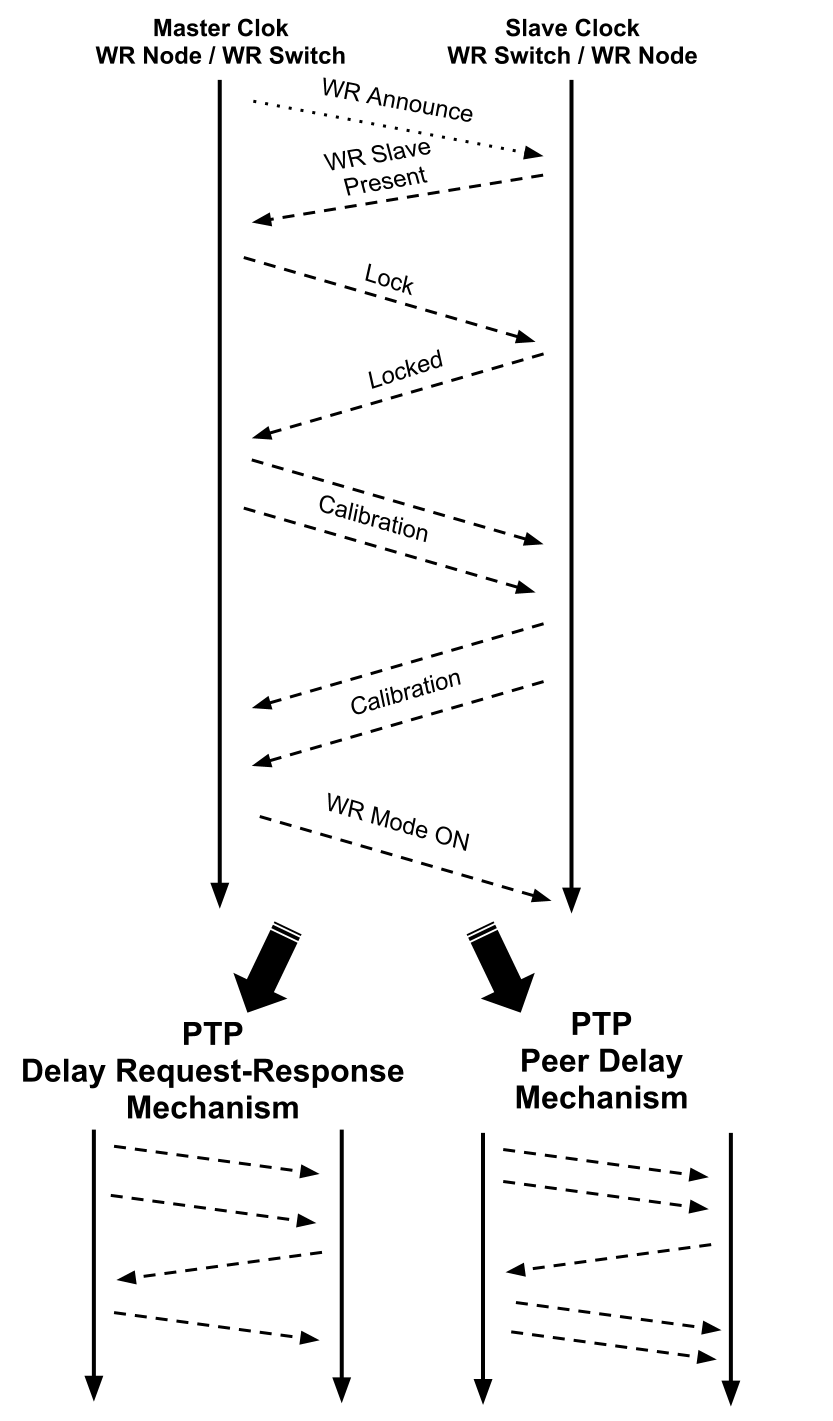
\includegraphics[scale=0.25]{fig/wr_ptp.png}
\caption{WR PTP Message Flow and PTP}
\label{fig:wr_ptp}
\end{figure}

%\FloatBarrier

